\documentclass[10pt,twocolumn]{article}
\usepackage[a4paper,margin=16mm,top=16mm,bottom=18mm]{geometry}
\usepackage[T1]{fontenc}
\usepackage{lmodern}
\usepackage{microtype}
\usepackage{booktabs}
\usepackage{amsmath}
\usepackage{tikz}
\usetikzlibrary{arrows.meta,positioning}
\usepackage{graphicx}
\usepackage{url}
\usepackage[hidelinks]{hyperref}
\usepackage{caption}
\captionsetup{font=small,labelfont=bf,skip=4pt}
\setlength{\columnsep}{7mm}
\setlength{\parskip}{0pt}
\setlength{\textfloatsep}{8pt}
\setlength{\intextsep}{8pt}
\setlength{\dbltextfloatsep}{8pt}
\usepackage{titlesec}
\titlespacing*{\section}{0pt}{7pt}{3pt}
\titlespacing*{\subsection}{0pt}{5pt}{2pt}
\titleformat*{\section}{\large\bfseries}
\titleformat*{\subsection}{\normalsize\bfseries}
\newcommand{\code}[1]{\texttt{\small #1}}

\title{\LARGE Parallel Place-and-Route of FINN Dataflow Accelerators\\[2pt]
\LARGE with a Static DFX Tile Overlay on the Alveo U55C\thanks{Code: FINN repository, branch \code{feature/rwislands}; log of all findings in \code{experiments/dynarapid/NOTES\_ISLANDS.md}.}}
\author{Lukas Stasytis\\TU Darmstadt\\[1pt]{\small Report, 12 October 2026}}
\date{}

\begin{document}
\maketitle

\begin{abstract}
\noindent
FINN compiles quantized neural networks into one streaming kernel per layer and hands the
stitched design to Vivado for a single global place-and-route (P\&R). On an Alveo U55C at
300\,MHz this takes hours for finn-examples models and frequently fails timing. We describe a
back end without a global step. The accelerator region of a cached shell is floorplanned once
into a serpentine of clock-region tiles, each a DFX reconfigurable partition, joined by fixed,
register-anchored link bundles. Per model, layers are synthesized out of context in parallel,
packed onto tiles, and each tile is placed, routed and written as a partial bitstream
independently. On a 64-core EPYC server, with 48 threads per build, VGG10 at 8$\times$ folding
builds in 1278\,s and meets 300\,MHz timing in every tile, against 8619\,s (timing failed) for
FINN's Vivado flow and 5176\,s for a baseline with the same parallel synthesis and shell but
one global P\&R; MobileNetV1 builds in 1541\,s against 6222\,s. The Vivado baselines at
300\,MHz ran on 8 cores (Vivado's default thread cap is 8), which is a threat to these ratios.
We also report an earlier RapidWright-stitched island flow (1.8--2.7$\times$ at 100\,MHz, fails
at 300\,MHz), what was verified and what was not, the bugs that verification found, and the
overlay's capacity limits.
\end{abstract}

\section{Introduction}
FINN~\cite{finn} emits a dataflow graph (DFG) of hardware nodes (matrix-vector units, MVAU;
thresholding; sliding-window generators; FIFOs; data-width converters; IODMAs) connected by
AXI-Stream channels with ready/valid handshakes. The graph is latency-insensitive: only
throughput matters, so any amount of pipelining may be inserted on a channel. The stock back
end stitches all nodes into one IP, synthesizes the whole design and runs one global
opt/place/phys\_opt/route in Vivado. On the xcu55c this scales poorly: the larger designs
measured here (300--400\,k LUTs, up to 5000 DSPs) take 6200--10600\,s at 300\,MHz and three of five fail
timing (Table~\ref{tab:300}). Vivado's placer and router by default use at most 8 threads, so
a 64-core server is mostly idle.

The goal set for this work was an order-of-magnitude reduction of bitstream turnaround through
parallel P\&R of independent parts of the design, at the cost of some area efficiency, with
functional correctness and timing at the target clock preserved. Cold builds are the normal case
(folding, FIFO sizes or quantization change between iterations), so the gain must come from
parallelism, not from reuse.

Contributions. (1)~A \emph{static tile overlay}: a cached DFX floorplan of the accelerator
region with pre-routed, anchored links (Section~\ref{sec:overlay}). (2)~A per-model flow that
runs OOC synthesis, tile assignment and tile implementation in parallel and produces one partial
bitstream per tile without any whole-design step. (3)~Credit-based pipelined links whose FIFO
depth is derived from the round-trip register count, with a simulation test. (4)~Measurements
of four flows on three finn-examples models at 100 and 300\,MHz, a functional verification
procedure, and an account of the bugs it caught and of the overlay's limits.

\section{Background and related work}
\textbf{Partition-based parallel P\&R.} RapidStream~1.0~\cite{rs1} splits a TAPA dataflow design
into 32 islands on a U250, places one anchor register per inter-island net in thin anchor
regions, implements the islands in parallel with Vivado, stitches with
RapidWright~\cite{rapidwright} and routes the 5--10\,\% conflicting nets globally (Vivado or
RWRoute~\cite{rwroute}); 5--7$\times$ over Vivado. RapidStream~2.0~\cite{rs2} removes the global
route: islands become DFX reconfigurable partitions routed in abstract shells against pre-routed
partition pins; 5.1--7.5$\times$ on a U280. RapidPnR~\cite{rapidpnr} shows the ceiling of plain
partition-and-merge without anchors (1.6--2.5$\times$).

\textbf{Page and overlay flows.} PRflow~\cite{prflow} and DW~\cite{dw} pre-build an interconnect
(packet NoC, pipelined links through PR switchboxes) between fixed PR pages; PLD~\cite{pld} nests
22 pages with abstract shells inside the Vitis shell (4.2--7.3$\times$ vs Vitis);
HiPR~\cite{hipr} uses one-clock-region tiles per function; hierarchical pages~\cite{hpages}
merge neighbours with nested DFX. Their shared lesson, which we follow: any post-hoc global route
caps the speedup; pre-routed interfaces or reuse are needed for an order of magnitude.

\textbf{Pre-implemented blocks.} DynaRapid~\cite{dynarapid} places a library of pre-implemented
relocatable components and routes with RWRoute (about 20$\times$ vs Vivado \emph{Quick}), but
only pays off with library reuse (library build about 10\,h). Our earlier flow used it and
dropped it for the cold-build reason above.

\textbf{Position.} The overlay is closest to RapidStream~2.0 and PLD: DFX tiles in abstract
shells, fixed anchored links, no global route. Differences: FINN dataflow as the input; a
serpentine grid sized to clock regions with static gaps; credit-based pipelined links with
transit registers through intermediate tiles; the static design cached per shell and clock; and
Tcl pre-placement of the grey-box placeholders, without which grey-box detail placement takes
tens of minutes and stalls beyond about 16 tiles.

\section{System}
\subsection{Shell}
The shell (PCIe XDMA, HBM/AXI interconnect, clocking) is implemented once per (board, clock,
IODMA interface), locked and cached (\code{dynarapid/shell.py build\_shell}). The accelerator
(\code{finn\_accel\_core}) is a black-box cell inside it. Every shell$\leftrightarrow$core
channel passes a two-entry register slice (\code{rwi\_bridge\_slice}) whose \code{ready} is driven
directly by a register, so the shell side of every boundary path is a flop. All flows compared
below use this shell, the same FINN front end and the same folding.

\subsection{Static overlay}
\label{sec:overlay}
\begin{figure}[t]
\centering
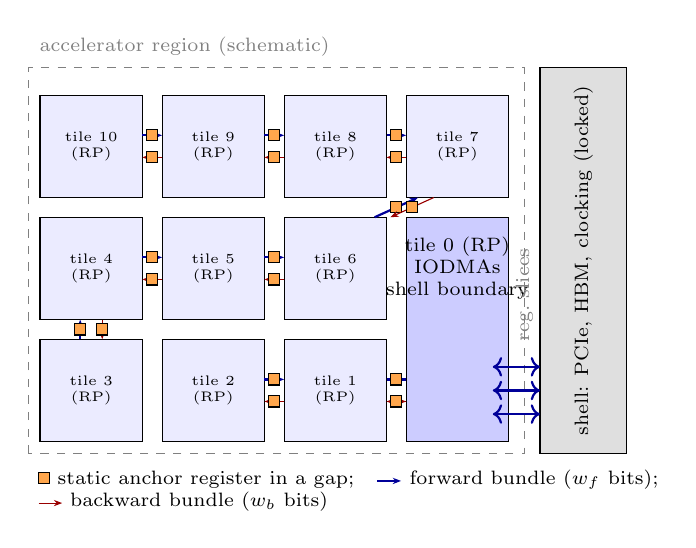
\begin{tikzpicture}[x=1cm,y=1cm,font=\scriptsize,
  ff/.style={draw,fill=orange!70,minimum width=4pt,minimum height=4pt,inner sep=0pt},
  lk/.style={-{Stealth[length=3pt]},thick,blue!60!black},
  bk/.style={-{Stealth[length=3pt]},thin,red!60!black}]
% shell on the right
\draw[fill=gray!25] (6.5,0) rectangle (7.6,4.9);
\node[rotate=90] at (7.05,2.45) {shell: PCIe, HBM, clocking (locked)};
% accelerator region frame
\draw[dashed,gray] (0,0) rectangle (6.3,4.9);
\node[anchor=south west,gray] at (0.02,4.92) {accelerator region (schematic)};
\def\tw{1.3}\def\th{1.3}\def\gx{0.25}\def\gy{0.25}
\foreach \c/\r/\k in {2/0/1, 1/0/2, 0/0/3, 0/1/4, 1/1/5, 2/1/6, 3/2/7, 2/2/8, 1/2/9, 0/2/10}{
  \pgfmathsetmacro{\x}{0.15+\c*(\tw+\gx)}
  \pgfmathsetmacro{\y}{0.15+\r*(\th+\gy)}
  \draw[fill=blue!8] (\x,\y) rectangle (\x+\tw,\y+\th);
  \node[align=center,font=\tiny] at (\x+0.5*\tw,\y+0.5*\th) {tile \k\\(RP)};
}
% tile 0: two rows high, next to the shell
\draw[fill=blue!20] (0.15+3*1.55,0.15) rectangle (0.15+3*1.55+1.3,0.15+2*1.3+0.25);
\node[align=center] at (0.15+3*1.55+0.65,2.35) {tile 0 (RP)\\IODMAs\\shell boundary};
\foreach \yy in {0.5,0.8,1.1}{\draw[lk,<->] (6.5,\yy) -- (5.9,\yy);}
\node[rotate=90,gray,anchor=west] at (6.3,1.3) {reg.\ slices};
% horizontal neighbours
\foreach \c/\r in {2/0, 1/0, 0/1, 1/1, 2/2, 1/2, 0/2}{
  \pgfmathsetmacro{\xa}{0.15+\c*(\tw+\gx)+\tw}
  \pgfmathsetmacro{\yc}{0.15+\r*(\th+\gy)+0.5*\th}
  \draw[lk] (\xa,\yc+0.14) -- (\xa+\gx,\yc+0.14); \node[ff] at (\xa+0.5*\gx,\yc+0.14) {};
  \draw[bk] (\xa+\gx,\yc-0.14) -- (\xa,\yc-0.14); \node[ff] at (\xa+0.5*\gx,\yc-0.14) {};
}
% tile0 -> tile1
\draw[lk] (0.15+3*1.55,0.15+0.65+0.14) -- (0.15+2*1.55+1.3,0.15+0.65+0.14); \node[ff] at (0.15+2*1.55+1.3+0.125,0.15+0.65+0.14) {};
\draw[bk] (0.15+2*1.55+1.3,0.15+0.65-0.14) -- (0.15+3*1.55,0.15+0.65-0.14); \node[ff] at (0.15+2*1.55+1.3+0.125,0.15+0.65-0.14) {};
% vertical turn tile3->4
\foreach \c/\r in {0/0}{
  \pgfmathsetmacro{\xc}{0.15+\c*(\tw+\gx)+0.5*\tw}
  \pgfmathsetmacro{\ya}{0.15+\r*(\th+\gy)+\th}
  \draw[lk] (\xc-0.14,\ya) -- (\xc-0.14,\ya+\gy); \node[ff] at (\xc-0.14,\ya+0.5*\gy) {};
  \draw[bk] (\xc+0.14,\ya+\gy) -- (\xc+0.14,\ya); \node[ff] at (\xc+0.14,\ya+0.5*\gy) {};
}
% diagonal turn tile6->7 (the slot above tile 0 left the serpentine)
\draw[lk] (4.4,3.0) -- (4.95,3.25); \node[ff] at (4.675,3.125) {};
\draw[bk] (5.15,3.25) -- (4.6,3.0); \node[ff] at (4.875,3.125) {};
% legend
\node[anchor=north west,align=left] at (0,-0.08) {\tikz\node[ff]{}; static anchor register in a gap;\quad
  \tikz\draw[lk](0,0)--(0.3,0); forward bundle ($w_f$ bits);\\ \tikz\draw[bk](0,0)--(0.3,0); backward bundle ($w_b$ bits)};
\end{tikzpicture}
\caption{Static overlay (schematic, 11 of 22 tiles): tile RPs along the serpentine with anchored link bundles in the gaps; tile 0 absorbs the slot above it, so the 6$\to$7 edge crosses diagonally.}
\label{fig:overlay}
\end{figure}

The overlay (\code{rwislands/overlay.py}, Fig.~\ref{fig:overlay}) is built once per (shell,
tile grid, link widths) and cached under a key that also includes the overlay version and the
Vivado release; we call the cached artefact the \emph{static overlay} and the locked, routed
design it contains the \emph{static design}. The accelerator region beside the shell is cut into
a serpentine (boustrophedon; ``snake'' in the code) of tiles aligned to clock regions. The
production grid is 22 tiles of 2$\times$2 clock regions (knobs \code{rows=120, crs=2}), tile~0
next to the shell being taller (\code{boundary\_rows}) because it carries the IODMAs and all
shell boundary signals. Each tile is a DFX reconfigurable partition (RP: a cell whose contents,
the reconfigurable module, RM, are implemented separately and loaded by a partial bitstream;
\code{HD.RECONFIGURABLE}, \code{SNAPPING\_MODE ON}) with its own pblock. Pblocks are shrunk by one
column and one or two rows on every side: the resulting \emph{gaps} are static channels that
hold the anchor registers and keep RP edges off clock-region boundaries (Vivado warns of limited
routability there).

\textbf{Links.} Serpentine edge $k$ (tile $k\leftrightarrow k{+}1$) carries a forward bundle of
$w_f$ bits and a backward bundle of $w_b$ bits. Every bit passes exactly one static \emph{anchor
register} (RapidStream's term; DW's relay station) in the gap, so each RP boundary net has one
static driver or load and one \emph{partition pin} (the fixed routing node at which a net
crosses the RP boundary), and every tile can be timed completely on its own. The production
overlay uses $w_f=2304$, $w_b=32$ (VGG10~8$\times$ needs 2151/15 bits); a second 22-tile overlay
with 1088/128 served the 100\,MHz VGG10 0.25$\times$ runs. Because tile~0 abuts the shell, its
boundary is timed against the bridges' register slices and needs no anchors.

\textbf{Reset.} The shell reset reaches the tiles through a static register chain along the
serpentine (one register per edge) plus one \code{DONT\_TOUCH} register per tile, again so that
each RP boundary net has a single static driver (a 14.7\,ns flat wire to far tiles failed setup,
and synthesis merging equivalent registers violated the DFX rule Constraints 18-4430).

\textbf{Grey boxes and the static build.} The tiles are filled with \emph{grey boxes} (a
placeholder RM: one \code{DONT\_TOUCH} LUT1 per port bit and one FDCE on the clock) so that the
static design can be placed, routed and locked with real partition pins. Vivado's detail placer
scales super-linearly on these tens of thousands of unconnected LUTs (29\,min for one phase with
24 tiles); \code{PLACE\_GREYBOX\_TCL} pre-places every link's LUTs on the slices nearest the
neighbouring tile before \code{place\_design}, which pulls the partition pins to that edge
(22 tiles: 5.5\,min, 79 tiles: 17\,min). The kernel clock net of the locked shell spans only the
clock regions of its old loads; it is unrouted and re-routed under DFX rules. The static design is
placed, routed, locked (\code{lock\_design -level routing}), written as a full bitstream, and one
\emph{abstract shell} per tile (a checkpoint reduced to the static logic and routing a single RP
needs for timing, \code{write\_abstract\_shell}) is written, 8 Vivado sessions in parallel.
\code{write\_bitstream} fails with more than 32 RPs in a design (Designutils 20-1700, Vivado
2024.2 and 2025.1), so the serpentine is cut at 32 tiles. One-off cost for 22 tiles on a shared
16-core lane: static 1050--1381\,s plus abstract shells 677--1031\,s; the shell itself about
950\,s at 300\,MHz. The static design closes timing at 100 and 300\,MHz (300\,MHz: worst
negative slack WNS +0.29/+0.26\,ns, worst hold slack WHS +0.009/+0.010\,ns, 0 routing errors).

\subsection{Per-model flow}
\code{flow.py \_overlay\_build} runs the following steps. Steps 2 and 6 run in parallel; the
planning steps 3--5 are serial but take seconds; nothing touches the whole design.
\begin{enumerate}\setlength{\itemsep}{0pt}
\item FINN front end output (folded, FIFO-sized dataflow ONNX) $\to$ \code{ZynqBuild}: IODMA
insertion, partitions, HLS IP synthesis (one flat pool of spawned processes over all HLS nodes).
\item \emph{Parallel OOC synthesis} of every distinct node (\code{synth\_design}, single-threaded
jobs, longest first; cheap FIFO/DWC/padding nodes batched in shared sessions; checkpoints cached
per content hash). Optional \emph{layer splitting} (\code{SplitLargeMVAU}) so that every part fits a
tile (knob \code{part}: 45\,\% of a median tile by default).
\item \emph{Tile assignment} (\code{plan\_overlay}): nodes in DFG order along the serpentine;
consecutive nodes share a tile while their synthesized utilization fits (LUT utilization tried
0.5--0.9; DSP/BRAM/URAM at \code{hard} = 90--95\,\% of the tile's sites); the IODMAs go to
tile~0. A node larger than every tile fails the plan with the reason.
\item \emph{Link plan} (\code{link\_plan}): every inter-tile stream gets a bit range on every
edge it crosses (data+valid in the forward bundle, ready in the backward one); tiles in between
pass it through. Bundle overflow fails the plan early.
\item \emph{Tile netlists} (\code{tile\_verilog}): a structural netlist per used tile, the member
nodes plus one link transmitter per outgoing and one receiver per incoming stream and pass-through
registers in transit tiles, linked with \code{link\_design} from the OOC checkpoints (no global
synthesis).
\item \emph{Tile implementation in parallel} (\code{tile\_tcl}): open the tile's abstract shell,
\code{read\_checkpoint -cell} the netlist into the RP, opt/place/phys\_opt/route with the
baseline's directives, reports, \code{write\_bitstream -cell} (the partial bitstream), and the
routed RM checkpoint. Threads per tile = lane threads / used tiles (2 on a 48-thread lane with 22
tiles).
\item Result: the cached static full bitstream plus one partial bitstream per used tile. No
assembly step; for verification only, the static design and all routed RMs are read into one
design to write a functional netlist.
\end{enumerate}

\subsection{Credit-based links}
\label{sec:links}
A link (\code{links.py}) is latency-insensitive with credit-style flow control. The transmitter
registers data and valid through $P_O$ output stages and the incoming ready through $P_I$
stages; the receiver registers inputs through $R_I$ stages into a FIFO and sends ready = ``at most
$\mathrm{DEPTH}-\mathrm{SLACK}$ words buffered'' through $R_O$ stages. Since ready is late, the
receiver must absorb every word in flight after it drops ready:
\[
\text{in flight} = P_O{+}P_I{+}R_I{+}R_O + 2e + 2(e{-}1)\,T ,
\]
for a link over $e$ edges (one anchor per edge and direction) with $T$ registers per transit
tile and direction. The FIFO depth is the smallest power of two $\ge 8$ with
$\mathrm{depth}-3 \ge$ in flight. The knob \code{pipe}$=p$ sets $P_O{=}P_I{=}R_O{=}p$,
$R_I{=}T{=}p{-}1$ (so $p{=}1$ gives $3+2e$); higher $p$ buys timing margin at the cost of FIFO depth
only, since inter-node latency is irrelevant in FINN dataflow. An xsim testbench over 1 and 3
edges with $p\in\{1,2,3\}$, random producer stalls and consumer back-pressure shows 0
lost, duplicated or reordered words at 1.000--1.008 cycles per word.

\subsection{The earlier island flow}
\label{sec:islands}
The island flow (\code{flow.py rw\_islands\_zynq\_build}, \code{IslandStitcher.java}) cuts the
DFG into islands, either a chain cut by min-max cost (\emph{Islands (chain)}) or a packing onto
16-column $\times$ 60-row clock-region tiles (\emph{Islands (grid)}), implements each island OOC
in its own pblock with \code{CONTAIN\_ROUTING} in parallel, with a two-entry register slice at
both ends of every inter-island stream, stitches the routed islands into the shell with
RapidWright (\code{populateBlackBox}, RWRoute partial routing of the inter-island nets with soft
preserve), and finishes with one Vivado assembly: read the routed core into the shell,
\code{route\_design} on the remaining nets, hold fix, bitstream. The assembly is a global step.
Islands (grid), VGG10~8$\times$, 100\,MHz: synthesis done at 352\,s, islands at 1011\,s,
stitching at 1425\,s, assembly at 2885\,s of 2947\,s, so stitching plus the global assembly is
about half the build (read core about 430\,s, route 1100--1400\,s, bitstream about 160\,s). At
300\,MHz the assembly starts with 4051 unrouted nets, runs three rip-up-and-reroute iterations
and ends at WNS $-3.842$\,ns (21\,894 failing endpoints): single-register crossings between
islands plus a global final route do not close timing at high $f_{\max}$, which motivated the
overlay.

\section{Codebase and integration}
The flow lives in \code{src/finn/util/rwislands/} (\code{overlay.py}: geometry, static Tcl, grey
boxes, tile and link plans, tile netlists and Tcl; \code{links.py}: link RTL and FIFO sizing;
\code{flow.py}: orchestration of all island-family flows; \code{floorplan.py}, \code{netlist.py},
\code{device.py}, \code{assembly.py}, \code{profiles.py}, \code{IslandStitcher.java} for the
island flow) and reuses \code{dynarapid/shell.py} (shell, bridges), \code{components.py} (node
synthesis, content-hash names, \code{FLOW\_VERSION}) and \code{tools.py} (\code{run\_vivado}:
machine-wide slot locks, memory gating, timeouts). Integration is one option of FINN's existing
transformation in \code{transformation/fpgadataflow/make\_zynq\_proj.py}:\\
\code{ZynqBuild(..., dynarapid=\{"flow": "islands",}\\
\code{\ \ "islands": "overlay"|"global"|"auto", "out\_dir",}\\
\code{\ \ "shell\_lib", "workers"\})}.\\
Overlay knobs come from the environment, e.g.\\
\code{FINN\_RWI\_OVERLAY="cols=16,rows=120,crs=2,}\\
\code{\ \ wf=2304,wb=32,gap\_rows=2,hard=95,pipe=2"};\\
grid and link widths are part of the overlay's cache key; \code{hard}, \code{part},
\code{pipe} and \code{tile0} are per-model knobs. Caches: shell per (board, clock, IODMA
interface); overlay per (shell, grid, link widths, overlay version, Vivado version); node
checkpoints per content hash and \code{FLOW\_VERSION}; link modules per width and depth.

Experiment scripts (\code{experiments/dynarapid/}): \code{run\_bitfile\_experiment.py} (one build,
\code{-{}-mode vivado|global|islands|overlay|overlay\_fast}), \code{run\_vshell\_timing.sh} (timed
builds, \code{runs.jsonl}), \code{run\_campaign.sh} (job queue over CPU lanes with disjoint
cores, per-lane Vivado slots, memory watchdog), \code{build\_overlay.py} (static overlay alone),
\code{verify\_accel.py} (functional check). Reproducing a point: build the shell and overlay once
with \code{build\_overlay.py}, then \code{run\_bitfile\_experiment.py -{}-mode overlay -{}-clk 3.333}
on the FINN dataflow ONNX with \code{-{}-shell-lib} pointing at the cached shells; every result
directory contains \code{result.json} with status, per-tile timing and stamps.

\section{Methodology}
\label{sec:method}
\begin{table*}[!t]
\centering\footnotesize
\caption{U55C, 300\,MHz: wall time in s, WNS in ns (shell and overlay cached).}
\label{tab:300}
\setlength{\tabcolsep}{3pt}
\begin{tabular}{@{}lllllr@{}}
\toprule
model & Vivado (FINN's flow) & Global & Islands (grid) & Overlay (\code{pipe=2}) & speedup vs Vivado \\
\midrule
VGG10 0.25$\times$ & 2511, +0.297 & -- & -- & 858, $\ge$+0.354 (3 tiles) & 2.9$\times$ \\
VGG10 8$\times$ & 8619, $-0.516$ fail & 5176, +0.227 & 3204, $-3.842$ fail & 1278, $\ge$+0.38 (22 tiles) & 6.7$\times$ (4.0$\times$ vs Global) \\
MobileNetV1 & 6222, 0.000 & 4305, $-0.033$ fail & 3491, $-5.408$ fail & 1541, $\ge$+0.129 (20 tiles) & 4.0$\times$ \\
VGG10 16$\times$ & 9820, $-0.188$ fail$^{a}$ & -- & -- & does not fit$^{b}$ & -- \\
ResNet50 & 10595, $-1.729$ fail & -- & -- & does not fit (12288-bit stream)$^{c}$ & -- \\
\bottomrule
\multicolumn{6}{@{}l@{}}{\footnotesize $^{a}$wrapper process killed by mistake; Vivado's implementation finished; time = job start to bitstream completion.} \\
\multicolumn{6}{@{}l@{}}{\footnotesize $^{b}$4994 DSP, greedy packing. $^{c}$a StreamingFIFO on a 12288-bit stream exceeds every tile and the 2304-bit bundles (Section~\ref{sec:limits}).}
\end{tabular}
\end{table*}
\begin{table}[!t]
\centering\footnotesize
\caption{U55C, 100\,MHz: wall time in s; all runs met timing.}
\label{tab:100}
\setlength{\tabcolsep}{3.5pt}
\begin{tabular}{@{}lrrrrr@{}}
\toprule
 & & & \multicolumn{2}{c}{Islands} & \\
\cmidrule(lr){4-5}
model & Vivado & Global & chain & grid & Overlay \\
\midrule
VGG10 0.25$\times$ & 2116 & 1168 & 918 & -- & 816 (2.6$\times$) \\
VGG10 8$\times$ & 6742 & 4351 & 3058 & 2947 & 1189 (5.7$\times$) \\
MobileNetV1 & 5287 & 3472 & 2940 & 2639 & not run \\
\bottomrule
\end{tabular}
\end{table}

\textbf{Machine.} AMD EPYC 9554P, 64 cores / 128 threads, 755\,GB RAM, Vivado 2024.2. The
machine is split into \emph{lanes} (disjoint sets of whole CCDs with their SMT siblings), one
timed job per lane: lanes A and B have 24 cores / 48 threads each and ran all parallel flows;
lane C (16 cores) is split into two 8-core / 16-thread sub-lanes for the Vivado baselines,
since Vivado uses at most 8 threads by default. \emph{Caveat:} the 300\,MHz Vivado baselines ran
on 8-core sub-lanes while the 100\,MHz ones ran on 48-thread lanes; a 48-thread rerun of the
300\,MHz VGG10~8$\times$ baseline was still running at the time of writing.

\textbf{What is timed.} Wall clock of the whole bitfile build from the FINN dataflow model: HLS,
synthesis, P\&R, bitstream. Shell and static overlay are cached and their one-off cost is
reported in Section~\ref{sec:overlay}; runs that had to build the shell or overlay were discarded
and rerun with warm caches. One run per point; earlier repeats showed about $\pm$5--10\,\%
variance.

\textbf{Flows.} \emph{Vivado} (FINN's flow): FINN's own \code{ZynqBuild} with the same shell
block design and Vivado's default directives (as Vitis v++): HLS, stitched IP, project synthesis,
one global opt/place/phys\_opt/route, bitstream. \emph{Global}: our parallel per-node OOC
synthesis and the cached shell, then one global P\&R of the core inside the shell; it isolates
the gain of parallel P\&R from that of parallel synthesis and the cached shell. \emph{Islands
(chain)} and \emph{Islands (grid)}: Section~\ref{sec:islands}. \emph{Overlay}: Section~\ref{sec:overlay}
with \code{pipe=2} at 300\,MHz.

\textbf{Models and metric.} finn-examples on the U55C: VGG10 RadioML at 0.25$\times$ folding
with residual adds (``0.25$\times$''), 8$\times$ and 16$\times$; MobileNetV1 (hand folding);
ResNet50. Synthesized sizes: VGG10~8$\times$ about 310\,k LUT and 4386 DSP (49\,\% of the
device's DSPs); VGG10~16$\times$ 404\,k LUT, 4994 DSP; MobileNet about 364\,k LUT (estimate) and
about 1150 BRAM. ``Met'' means 0 routing errors, WNS $\ge 0$ and WHS $\ge 0$; for Overlay
every tile and the static design must meet. Clocks: 100\,MHz (10\,ns) and 300\,MHz (3.333\,ns).

\section{Results}
\textbf{300\,MHz (Table~\ref{tab:300}).} Overlay is the only flow that meets timing on both
VGG10~8$\times$ and MobileNetV1; Global meets it on VGG10~8$\times$ and Vivado on MobileNet
(WNS exactly 0.000\,ns). Speedups over Vivado are 2.9$\times$ (VGG10 0.25$\times$), 6.7$\times$
(VGG10 8$\times$) and 4.0$\times$ (MobileNet); over Global, 4.0$\times$ on VGG10~8$\times$.
Global itself is 1.7$\times$ faster than Vivado on VGG10~8$\times$, which bounds what parallel
synthesis and the cached shell contribute; the remaining factor comes from parallel tile P\&R.
Islands (grid) is faster than Global but fails timing by 3.8--5.4\,ns because of its global final
route. VGG10~16$\times$ exceeds the overlay's usable DSP capacity and ResNet50 has a stream too wide
for a tile; both remain Vivado-only, and Vivado fails timing on both.

\textbf{100\,MHz (Table~\ref{tab:100}).} Overlay is 2.6$\times$ and 5.7$\times$ faster than
Vivado (VGG10 8$\times$ tiles at WNS $\ge$ +2.14\,ns); the island flows reach 1.8--2.3$\times$ and
Global 1.5--1.8$\times$. \code{overlay\_fast} (Vivado's RuntimeOptimized directives) on
VGG10~8$\times$ took 1230\,s, no gain over 1189\,s: per-tile placement costs about 350\,s
either way.

\textbf{Where the time goes.} VGG10~8$\times$ at 300\,MHz: the synthesis phase ends at 357\,s,
tiles take 449--846\,s each and all are done at 1203\,s; MobileNet: synthesis 586\,s, tiles
317--760\,s, done at 1346\,s; VGG10 0.25$\times$: synthesis 284\,s, tiles 282--509\,s. The
synthesis phase is throughput bound (MobileNet: 16.3\,k slot-seconds of single-threaded jobs on
32 Vivado slots; the longest node 160--180\,s). A typical tile (25--30\,k LUT, 256 DSP, 2
threads, 100\,MHz) spends: link 40\,s, open abstract shell 10\,s, read RM 25\,s, opt 45\,s,
place 350--450\,s (device and netlist model about 70\,s, global placement about 100\,s, detail
about 60\,s, post-placement about 90\,s), route 120--230\,s, partial bitstream about 50\,s.
The fixed per-tile costs (about 600\,s) plus the longest tile set the floor of the observed
800--1300\,s.

\textbf{Earlier island-flow results} (2026-10-07, 100\,MHz, previous FINN version, verified
models): ZCU104 TFC 644$\to$323\,s, CNV 891$\to$393\,s, VGG10 2112$\to$1205\,s; U55C TFC
1528$\to$722\,s, VGG10 2980$\to$1397\,s, MobileNet (U250 folding) 5424$\to$1989\,s: 2.0--2.7$\times$,
the ceiling of partition-and-merge with a global final route.

\section{Correctness and reliability}
\textbf{Verification method.} \code{verify\_accel.py} simulates in xsim the post-route functional
netlist of the core (for Overlay: the static design with all routed RMs read in) together
with the shell's bridge RTL, against FINN's stitched-IP RTL of the same graph, under one
SystemVerilog testbench that programs AXI-Lite like the FINN driver and models the AXI memories.
Inputs are random with per-frame amplitude scaling (\code{-{}-vary-amplitude}) so that frames fall
into different classes; the output buffers must be identical. A suspicious reference was
cross-checked against FINN's Python execution of the streamlined ONNX model.

\textbf{Verified:} VGG10 0.25$\times$ Overlay at 100\,MHz (8 frames covering 3 classes) and at
300\,MHz with \code{pipe=2} (8 frames, same classes); VGG10 0.25$\times$ Islands (4 frames);
VGG10~8$\times$ Overlay at 100\,MHz (2 frames, 2 classes; 3.5\,h of netlist simulation); earlier
TFC (16 frames) and VGG10 on the ZCU104 (8 frames). \textbf{Not verified:} the MobileNet Overlay
builds, any 300\,MHz VGG10~8$\times$ build, and on-board execution: partial reconfiguration was
not exercised on a board, only the assembled netlist was simulated.

\textbf{Bugs found by this process} (all fixed, with regression guards):
(1)~Thresholding units synthesized with all-zero threshold memories after a FINN upstream merge:
the HDL reads \code{.dat} files by a relative path that OOC synthesis did not find (only a critical
warning, Synth 8-4445); all non-Vivado results of two days were functionally wrong while their
timings barely changed after the fix. Init files are now copied into the synthesis directory,
Synth 8-4445 fails the node, and \code{FLOW\_VERSION} was bumped. (2)~Multi-edge links lost words
with a FIFO slack sized for one edge; reproduced in xsim, fixed by the round-trip formula of
Section~\ref{sec:links}. (3)~Reset setup failures and merged reset registers (Section~\ref{sec:overlay}).
(4)~The static \code{place\_design} stall and (5)~the 32-RP bitstream limit
(Section~\ref{sec:overlay}). (6)~FINN's own baseline failed for ResNet50 (\code{ip\_repo\_paths}
read back truncated); fixed. (7)~Earlier, in the island flow: SLR-crossing islands, a dropped
ElementwiseAdd input, a combinational bridge ready, partition cycles in the ResNet50 floorplan.

\textbf{Status gating.} Every flow result records a status; \code{ok} requires complete routing
and setup and hold met in every tile, and failures are reported as results (no silent fallback in
experiments). Cache keys include the flow version, the Vivado version and the knobs, so a changed
flow never reuses stale artefacts.

\section{Limitations and threats to validity}
\label{sec:limits}
\begin{itemize}\setlength{\itemsep}{0pt}
\item \emph{Capacity.} Tiles cover about 74\,\% of the device's DSPs (6720 of 9024; shell area
and gaps are lost), and greedy in-order packing wastes up to about 30\,\% in DSP-heavy tiles (two
128-DSP parts in a 368-DSP tile), so VGG10~16$\times$ (4994 DSP) does not fit. Vivado can use the
whole device.
\item \emph{Very wide streams.} ResNet50 has a StreamingFIFO on a 12288-bit stream (depth 2,
about 12.3\,k LUTs as LUTRAM) that is larger than every tile under the planner's limits, and the
stream is far wider than the 2304-bit bundles: such streams must stay inside one tile, which
needs a width converter or a different folding.
\item \emph{Floor.} The 32-tile cap bounds parallelism; per-tile fixed costs bound the build
time at the observed 800--1300\,s (Results).
\item \emph{One-off cost.} 35--40\,min per (shell, clock, grid); a new IODMA interface means a
new shell and overlay.
\item \emph{Fixed bundles.} A model whose streams exceed $w_f$/$w_b$ fails the plan early.
\item \emph{Measurement.} Single runs; 300\,MHz Vivado baselines on 8 cores vs 48 threads for
the parallel flows (Section~\ref{sec:method}); the 48-thread rerun was not finished.
\item \emph{Verification coverage.} MobileNet and 300\,MHz VGG10~8$\times$ Overlay builds
unverified; no on-board test; the partial-reconfiguration deployment path (programming the
static full bitstream and the partials on a U55C) not exercised.
\end{itemize}

\section{Future work}
TODO experiments: a ladder of longer Vivado jobs (ResNet50 on the overlay once its 12288-bit
stream is narrowed or kept inside a tile, its 100\,MHz Vivado baseline is running; VGG10~16$\times$
after capacity fixes); the 48-thread rerun of the 300\,MHz
VGG10~8$\times$ Vivado baseline (running); whole-machine runs (128 threads, about 5 threads per
tile) to measure scaling; functional verification of the MobileNet and 300\,MHz
VGG10~8$\times$ Overlay builds; an on-board test with partial bitstreams; the parked ZCU104 jobs
with the current flow.
Missing pieces: capacity (smaller split parts, \code{part=30}; compute nodes in tile~0, implemented
as knob \code{tile0}; tighter gaps; tiles over unused shell area; non-greedy packing); overlapping
synthesis with tile P\&R (start a tile when its members are synthesized) and synthesis on all lane
threads (48 instead of 32 slots); reuse of unchanged tiles' partial bitstreams across builds,
which DFX makes possible; and, for the island flow, credit-based pipelined links instead of
single-register crossings, or retiring it in favour of the overlay.

\begin{thebibliography}{9}\footnotesize\setlength{\itemsep}{0pt}
\bibitem{finn} Y. Umuroglu et al., FINN: a framework for fast, scalable binarized neural network inference, FPGA 2017.
\bibitem{rs1} L. Guo et al., RapidStream: parallel physical implementation of FPGA HLS designs, FPGA 2022.
\bibitem{rs2} L. Guo et al., RapidStream 2.0: parallel implementation of latency-insensitive FPGA designs with nested DFX, ACM TRETS 2023.
\bibitem{rapidpnr} RapidPnR: netlist-level partitioning into a grid of islands, parallel P\&R and merge, FCCM 2025 (poster).
\bibitem{prflow} D. Park, Y. Xiao, N. Magnezi, A. DeHon, PRflow: fast FPGA compilation using partial reconfiguration, FPL 2018.
\bibitem{dw} Y. Xiao, A. Ahmed, A. DeHon, DW: fast linking of separately compiled FPGA blocks without a NoC, FPT 2020.
\bibitem{pld} PLD: fast FPGA compilation with nested DFX pages inside the Vitis shell, ASPLOS 2022.
\bibitem{hipr} HiPR: high-level partial reconfiguration for fast incremental FPGA compilation, FPL 2022 / ACM TRETS 2023.
\bibitem{hpages} Hierarchical PR pages with nested DFX, FPT 2022.
\bibitem{dynarapid} DynaRapid: pre-implemented relocatable component library with RapidWright placement and RWRoute, FPL 2024.
\bibitem{rwroute} RWRoute: an open-source timing-driven router for commercial FPGAs, FPT 2021.
\bibitem{rapidwright} C. Lavin, A. Kaviani, RapidWright: enabling custom crafted implementations for FPGAs, FCCM 2018.
\bibitem{ug909} AMD, Vivado Design Suite User Guide: Dynamic Function eXchange (UG909); abstract shells.
\end{thebibliography}

\end{document}
